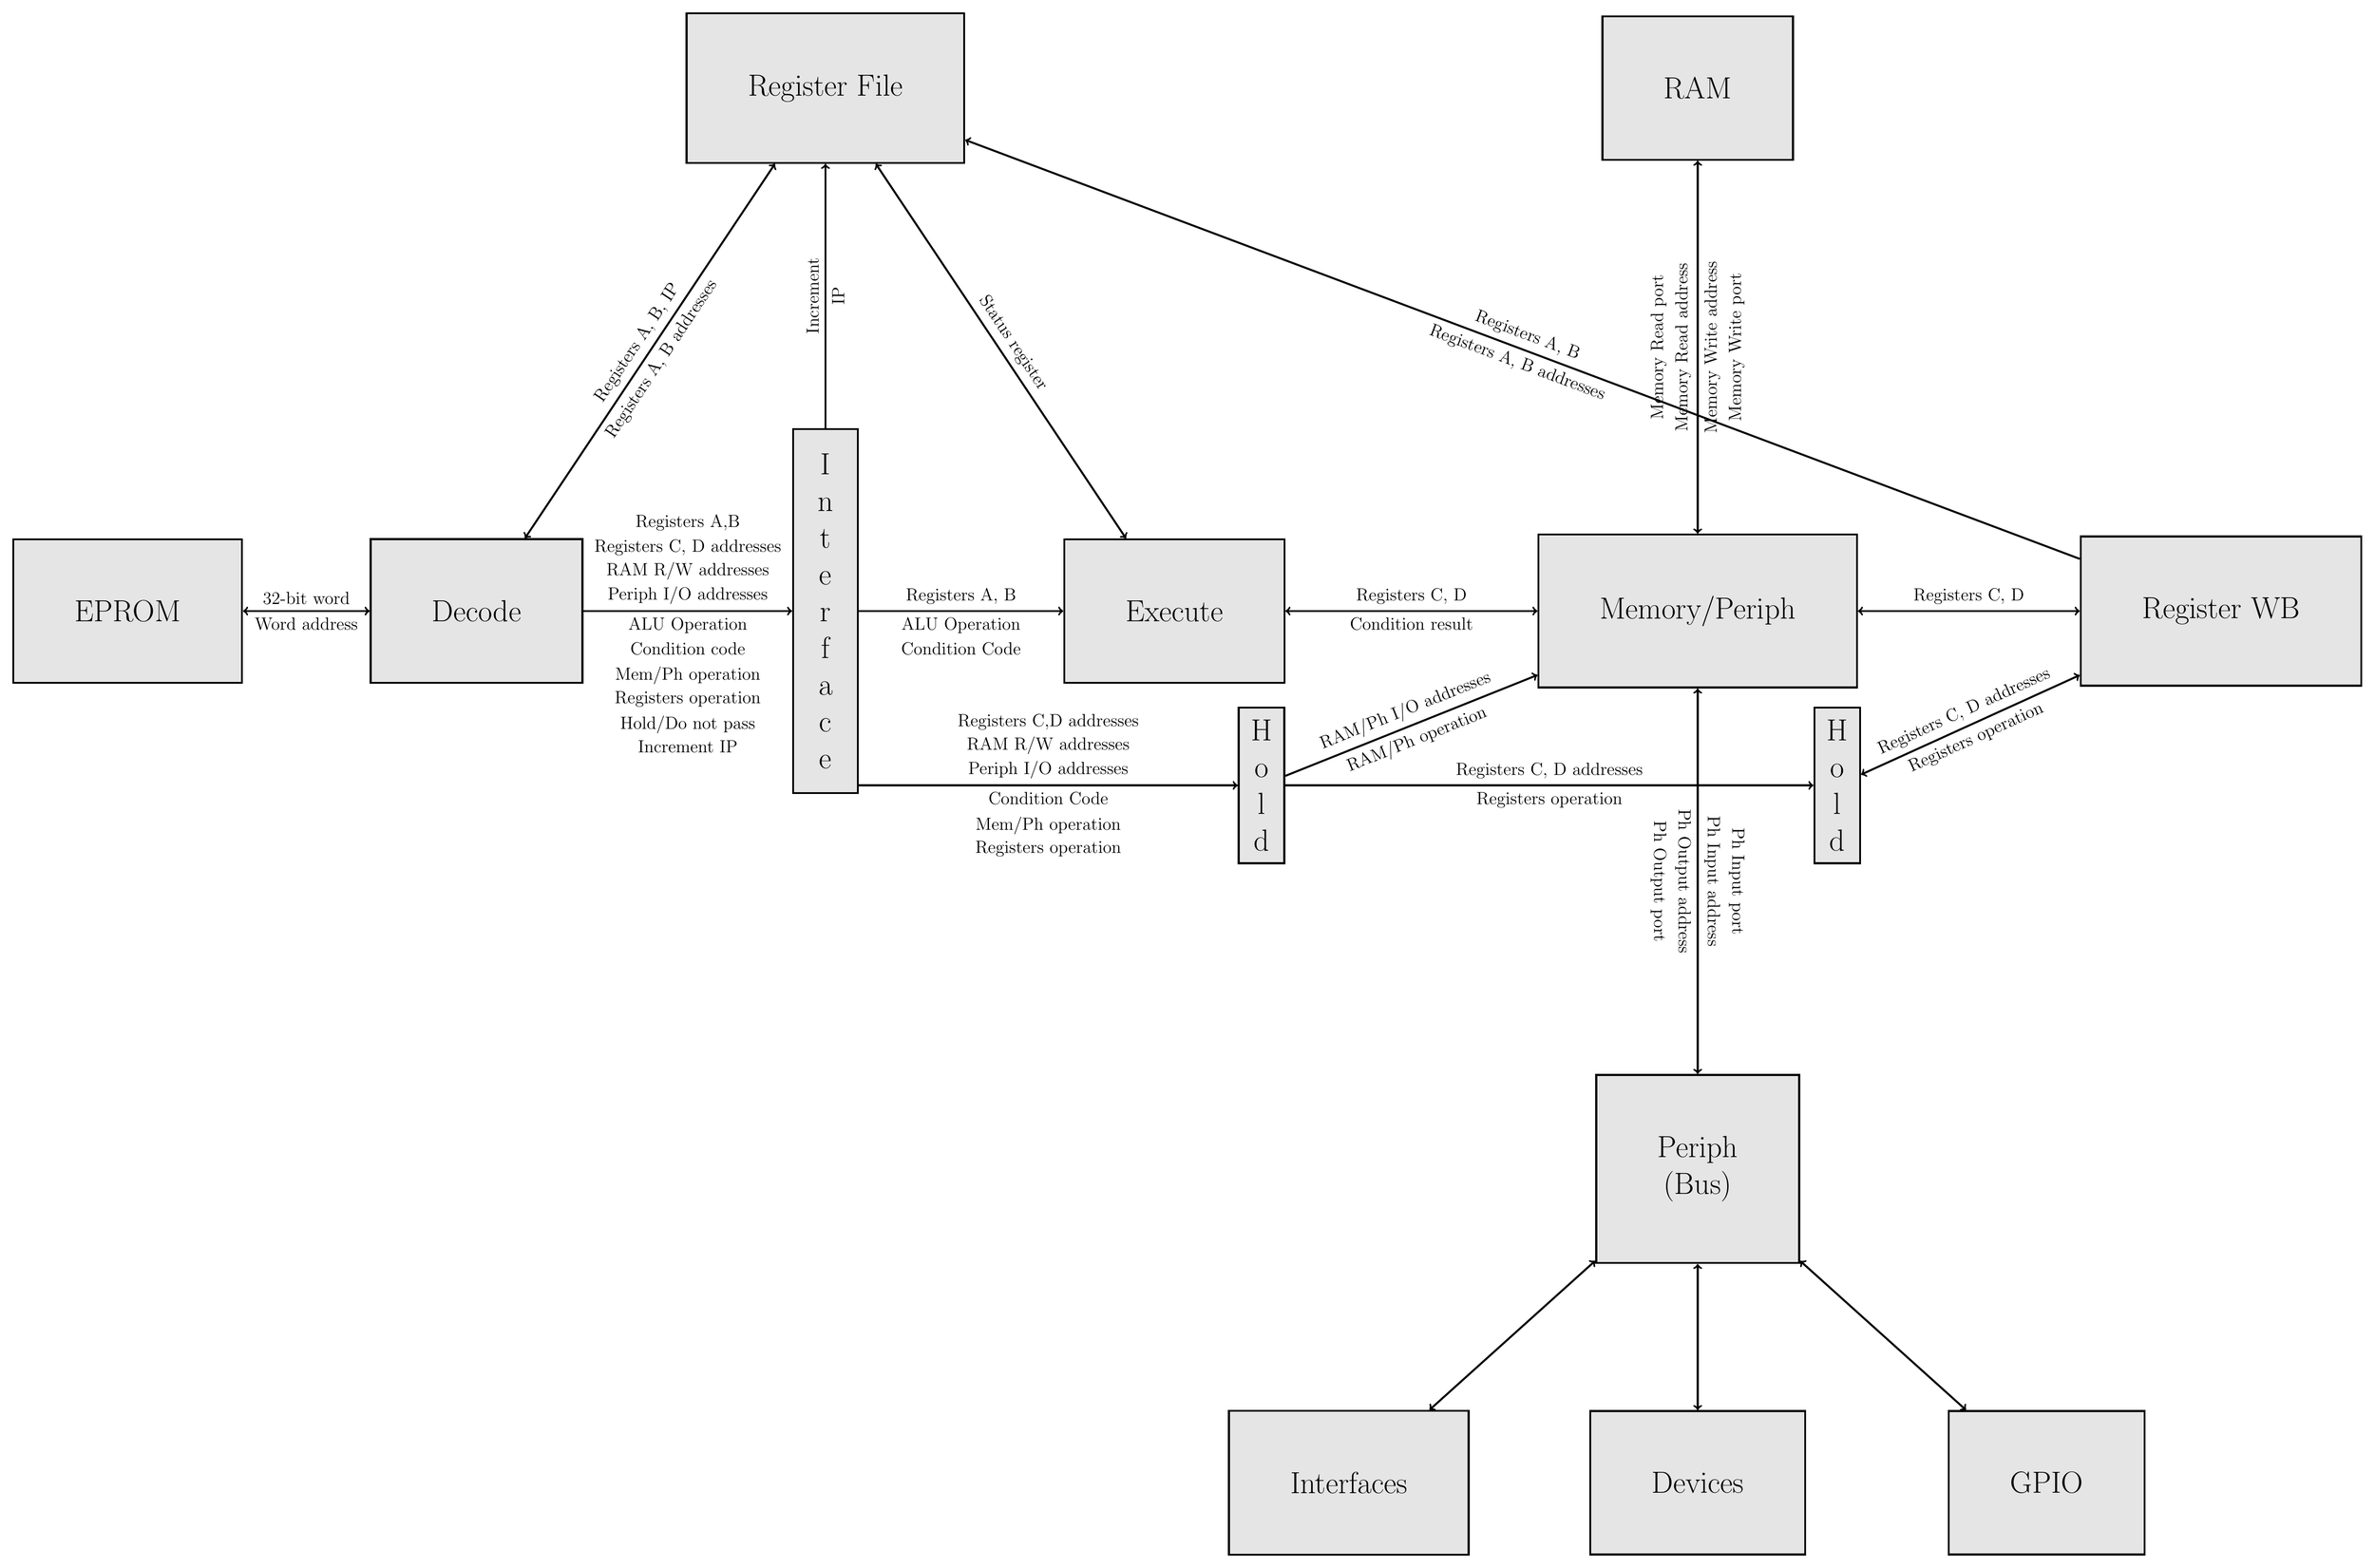
\begin{tikzpicture}[ultra thick, rect/.style={rectangle, draw=black,ultra thick, fill=gray!20, inner sep=#1, node font=\Huge, align=center}, rect/.default=50, arrownode/.style={pos=0.5, sloped, #1, node font=\Large}, arrownode/.default=above]

\node [rect] (RF) at (20, 15) {Register File};
\node [rect] (RAM) at (45, 15){RAM};
\node [rect] (P) at (0, 0){EPROM};
\node [rect] (D) at (10,0){Decode};
\node [rect=20] (I) at (20,0){I\\n\\t\\e\\r\\f\\a\\c\\e};
\node [rect] (EX) at (30,0){Execute};
\node [rect=10] (EXH) at (32.5,-5){H\\o\\l\\d};
\node [rect] (MEM) at (45,0){Memory/Periph};
\node [rect=10] (MEMH) at (49,-5){H\\o\\l\\d};
\node [rect] (WB) at (60,0){Register WB};
\node [rect] (PR) at (45, -16){Periph\\(Bus)};
\node [rect] (IF) at (35, -25){Interfaces};
\node [rect] (GP) at (55, -25){GPIO};
\node [rect] (DEV) at (45, -25){Devices};

\draw[<->,ultra thick] (P) -- (D) node [arrownode] { 32-bit word} node [arrownode=below] { Word address};
\draw[<->,ultra thick] (RF) -- (D) node [arrownode] {Registers A, B, IP} node[arrownode=below] {Registers A, B addresses};
\draw[->,ultra thick] (D) -- (I) node [arrownode={above=20}] {RAM R/W addresses} node [arrownode={above=40}] {Registers C, D addresses} node [arrownode={above=60}] {Registers A,B} node [arrownode={above=0}] {Periph I/O addresses}  node [arrownode={below=0}] {ALU Operation} node [arrownode={below=20}] {Condition code} node [arrownode={below=40}] {Mem/Ph operation} node [arrownode={below=60}] {Registers operation} node [arrownode={below=80}] {Hold/Do not pass} node [arrownode={below=100}] {Increment IP};
\draw[->,ultra thick] (I) -- (RF) node [arrownode] {Increment} node [arrownode=below] {IP};
\draw[->,ultra thick] (I) -- (EX) node [arrownode={above=0}] {Registers A, B} node [arrownode={below=0}] {ALU Operation} node [arrownode={below=20}] {Condition Code};
\draw[->,ultra thick] (I.east)+(0,-5) -- (EXH) node [arrownode={above=40}] {Registers C,D addresses} node [arrownode={above=20}] {RAM R/W addresses} node [arrownode={above=0}] {Periph I/O addresses} node [arrownode={below=0}] {Condition Code} node [arrownode={below=20}] {Mem/Ph operation} node [arrownode={below=40}] {Registers operation};
\draw[<->,ultra thick] (EX) -- (MEM) node [arrownode] {Registers C, D} node[arrownode=below] {Condition result};
\draw[<->,ultra thick] (EX) -- (RF) node [arrownode] {Status register};
\draw[->,ultra thick] (EXH) -- (MEM) node [arrownode] {RAM/Ph I/O addresses} node [arrownode=below] {RAM/Ph operation};
\draw[->,ultra thick] (EXH) -- (MEMH) node [arrownode] {Registers C, D addresses} node [arrownode=below] {Registers operation};
\draw[<->,ultra thick] (MEM) -- (RAM) node [arrownode={above=20}] {Memory Read port} node [arrownode={above=0}] {Memory Read address} node [arrownode={below=0}] {Memory Write address} node [arrownode={below=20}] {Memory Write port};
\draw[<->,ultra thick] (MEM) -- (PR) node [arrownode={above=20}] {Ph Input port} node [arrownode={above=0}] {Ph Input address} node [arrownode={below=0}] {Ph Output address} node [arrownode={below=20}] {Ph Output port};
\draw[<->,ultra thick] (MEM) -- (WB) node [arrownode] { Registers C, D };
\draw[<->,ultra thick] (MEMH) -- (WB) node [arrownode] { Registers C, D addresses} node [arrownode=below] { Registers operation};
\draw[->,ultra thick] (WB) -- (RF) node [arrownode] { Registers A, B} node [arrownode=below] { Registers A, B addresses};
\draw[<->,ultra thick] (PR) -- (IF);
\draw[<->,ultra thick] (PR) -- (GP);
\draw[<->,ultra thick] (PR) -- (DEV);

\end{tikzpicture}